\documentclass[14Q,twocolumn]{jsarticle}
\usepackage[dvipdfmx]{graphicx}
\usepackage{wrapfig}
\usepackage{float}
\usepackage{otf}
\usepackage{longtable}
\usepackage{ulem}
\usepackage{ascmac}
\usepackage{multicol}
%%%%%
\makeatletter
\newenvironment{tablehere}
  {\def\@captype{table}}
  {}
\newenvironment{figurehere}
  {\def\@captype{figure}}
  {}
\makeatother
%%%%%%
\setlength{\textwidth}{160truemm}      % テキスト幅: 160mm
\setlength{\fullwidth}{\textwidth}     % ページ全体の幅
\setlength{\oddsidemargin}{0mm}   % 左余白
\setlength{\topmargin}{-10mm}       % 上余白
\setlength{\textheight}{240truemm}     % テキスト高さ: 297-(30+30)=237mm
\pagestyle{empty}
\title{QGIS印刷編\\{\large 所在調査報告書をつくる}}% 文書のタイトル
\date{2018年9月18日}
\author{厚沢部町 石 井 淳 平}              % 著者

%------------------------------
\begin{document}
\maketitle
%\begin{multicols}{2}
\section{この時間に覚えること}
ベクタデータの扱い方をマスターします。ベクタデータはデータベースとしての側面があり、論理演算子を使用して色や線種などを指定することができます。データベースとしてのベクタデータの取り扱いを実習します。

また、QGISは印刷原稿を作成するための「レイアウト」という機能が用意されており、高品質な印刷原稿を作成することができます。調査成果などの日常的な出図にも役に立つ「レイアウト」機能を使った版組を実習します。

\begin{itemize}
\item ベクタデータを加工して線種変更、彩色をする
\item 演算子を使ったベクタデータの分類と表現
\item 「レイアウト」による印刷原稿の作成
\end{itemize}


%%%%
\section{座標参照系を変更する}
座標参照系(測地系や投影系の総称)を変更します。ダウンロードしたばかりのGISデータは普段使う座標参照系ではないことがほとんどです。そのため、GISをデータを使用するほとんどの場合には、座標参照系の変更を行います。特に緯度経度系のデータでは面積計算や距離計算をはじめとした空間演算処理ができないので必ず変更してください。

\begin{enumerate}
\item 「buildings」を右クリック
\item 「エクスポート」→「地物の保存」
\item  「座標参照系」を「JGD2000/UTM zone 54N」に変更
\item ファイル名を「buildings\_utm54」に変更
\end{enumerate}

\begin{figurehere}
\centering
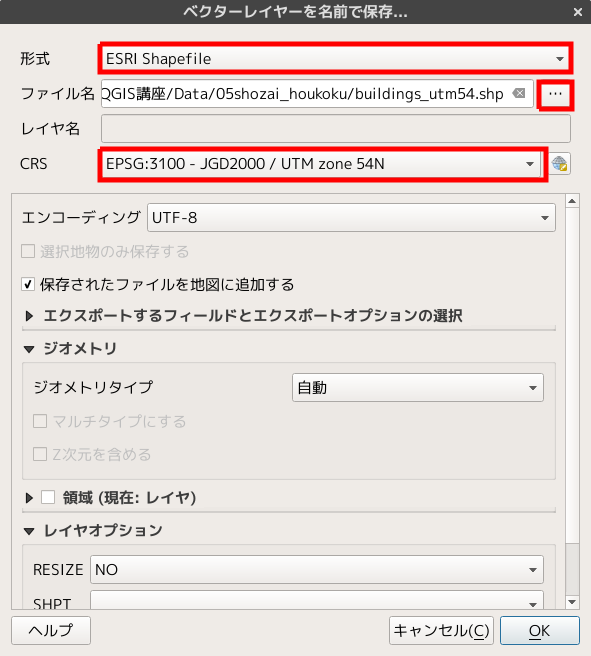
\includegraphics[width=0.5\linewidth]{04.png}
\caption{座標参照系をJGD2000/UTMzone54Nに変更する}
\end{figurehere}

%%%%
\section{ベクタデータの色や線種を変更}
\begin{enumerate}
\item 河川(WL\_polygon\_utm54)をダブルクリック
\item 「レイヤプロパティ」→「シンポロジ」
\item 「diagonal」(もともと用意されているデザインセット)を選択
\end{enumerate}

\begin{figurehere}
\centering
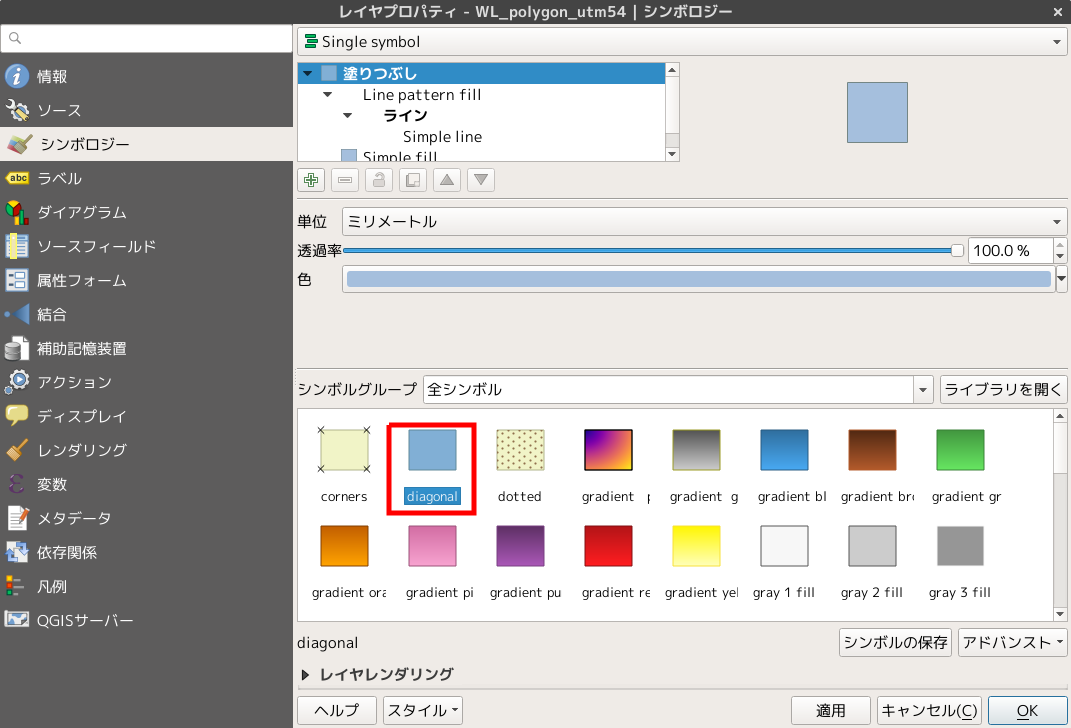
\includegraphics[width=1\linewidth]{05.png}
\caption{河川データの色と線種を指定}
\end{figurehere}

\begin{figurehere}
\centering
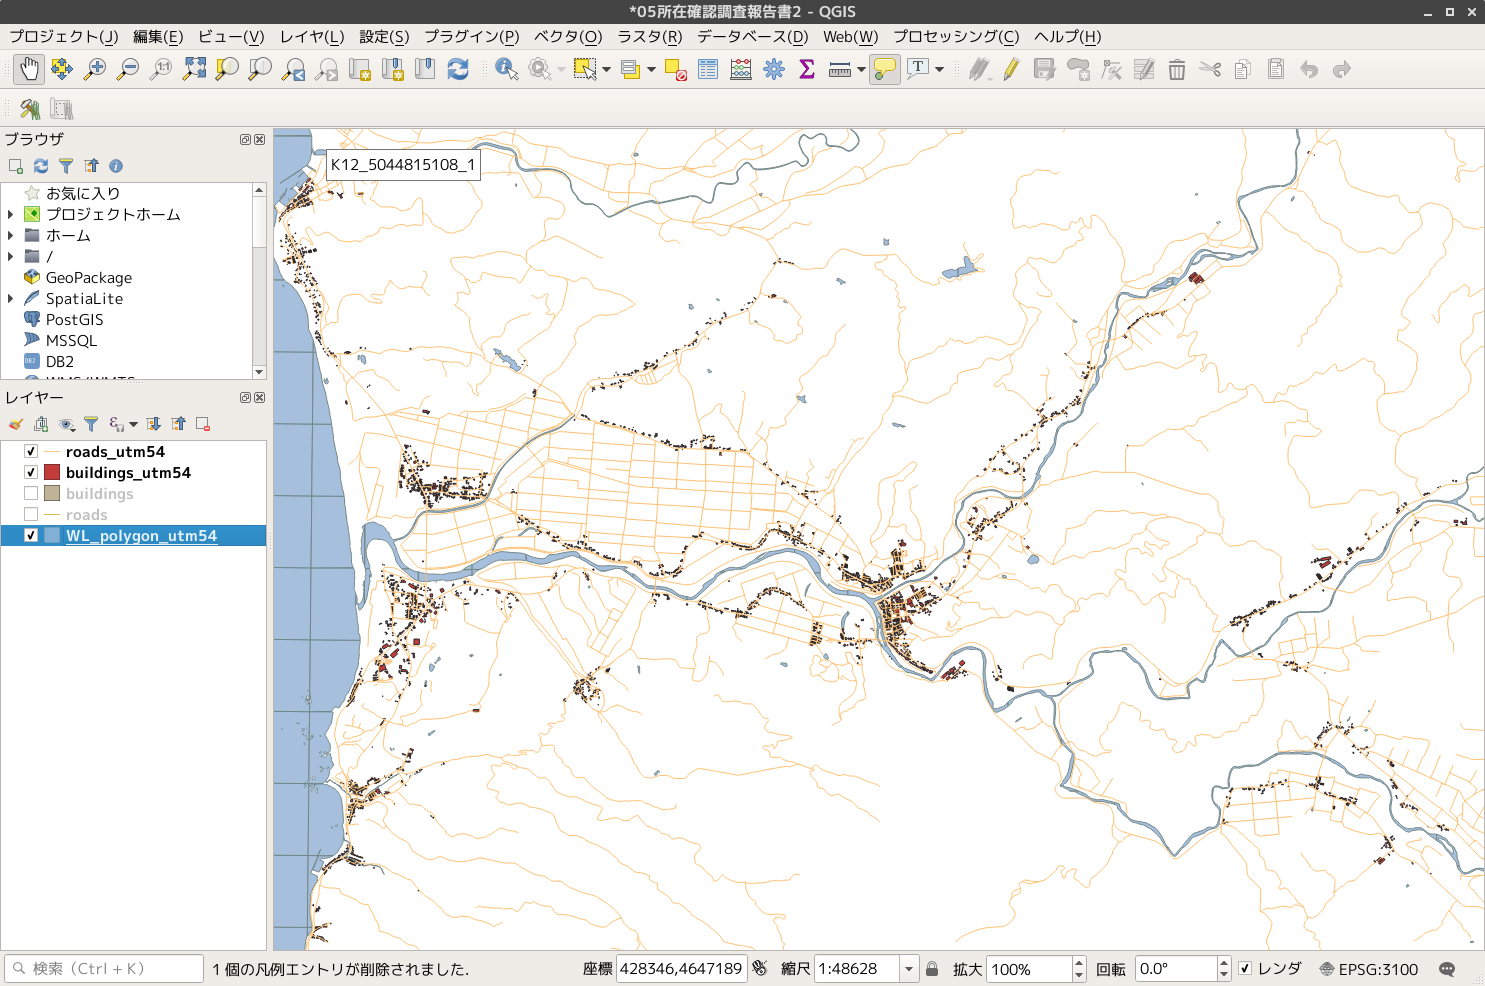
\includegraphics[width=1\linewidth]{06.png}
\caption{水域が水色に塗りつぶされる}
\end{figurehere}

%%%%
\section{分類ごとに色を変える}
「Categolized」を設定すると指定したフィールドの属性にあわせて自動的に分類されます。分類項目が適切で小数の場合には十分な結果が得られますが、分類が細かすぎる場合には適切な結果が得られないことが多くなります。

\begin{enumerate}
\item 道路データ(road)をダブルクリック
\item 「シンポロジー」→「Categolized」
\item 「カラム」→「タイプ」
\item  「分類」
\end{enumerate}

\begin{figurehere}
\centering
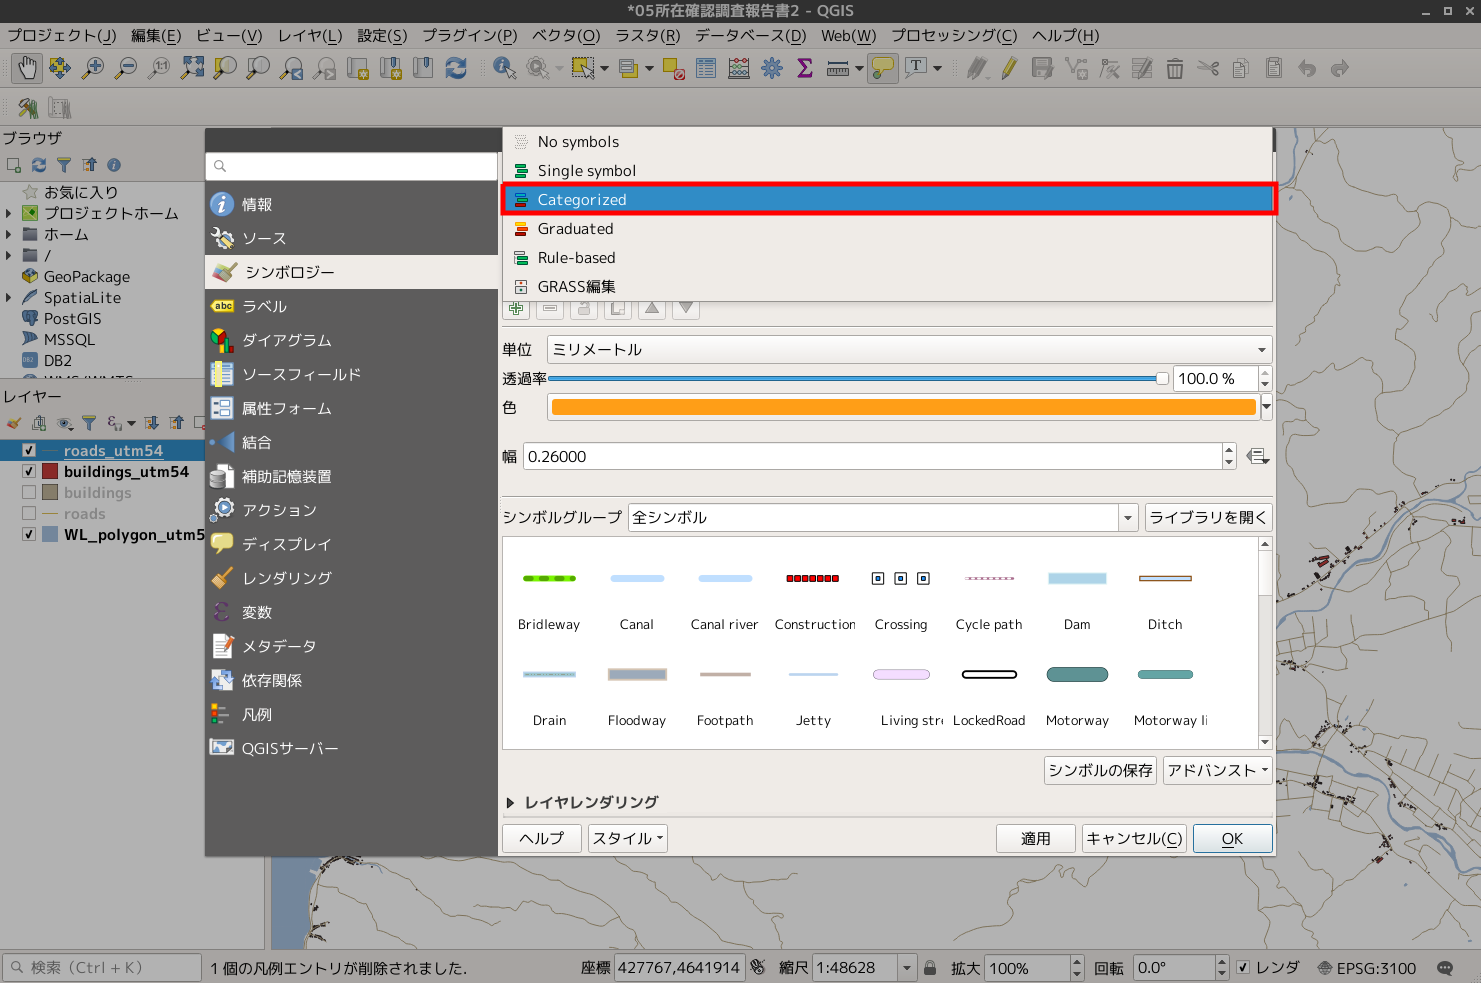
\includegraphics[width=1\linewidth]{07.png}
\caption{「Categolized」を選択する}
\end{figurehere}

\begin{figurehere}
\centering
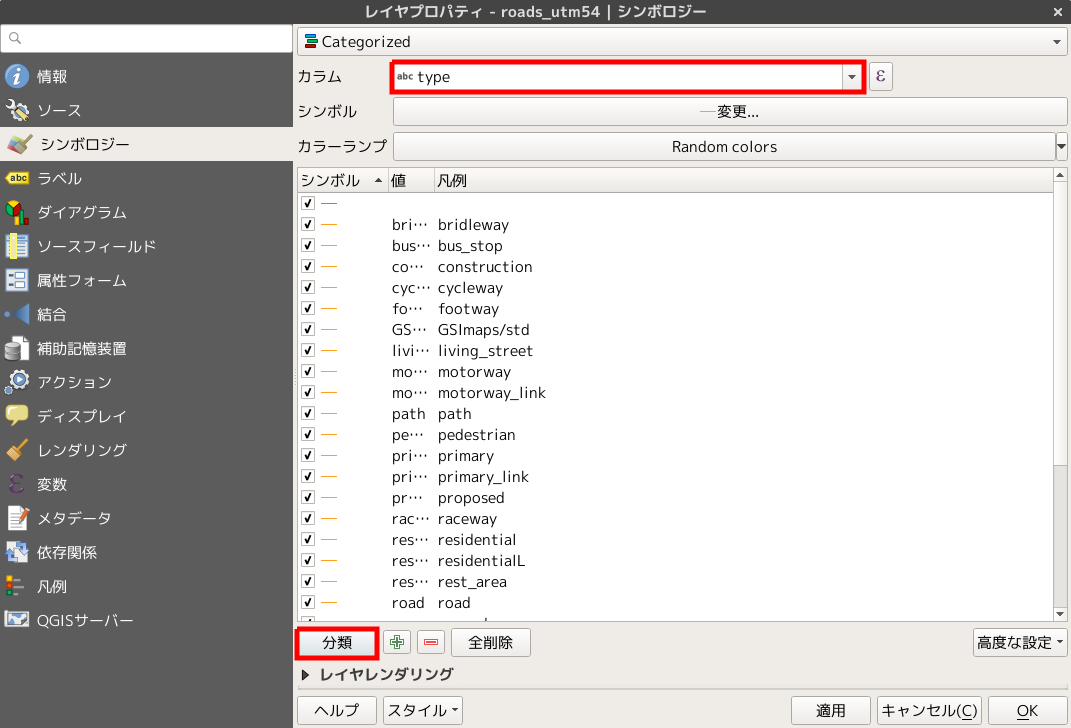
\includegraphics[width=1\linewidth]{08.png}
\caption{分類が細かすぎて分けきれない}
\end{figurehere}

%%%%
\section{論理演算子を使って色や線種を変える}
「Categolized」を使って自動的に分類すると分類数が多くなりすぎる場合や分類が不統一な場合には論理式を使用して手動で分類します。たとえば、縄文時代前期、縄文時代中期、旧石器時代などの時期区分がある場合、「縄文時代」という区分で分類する場合には「"時期区分" LIKE '\%縄文\%'」のように検索語を指定して縄文時代だけを抜き出すことが可能です。ベクタデータをデータベースとして活用する場合には必須の作業となりますので、確実にマスターしてください。

\begin{enumerate}
\item 「Ruleーbased」切り替え
\item 左下の「+」マークをクリックして条件を追加
\item 「色」→好きな色に変更
\item 「幅」→太め(1以上に 単位はミリ)
\item 「フィルター」に論理式を入力
\end{enumerate}

\newpage
\begin{figurehere}
\centering
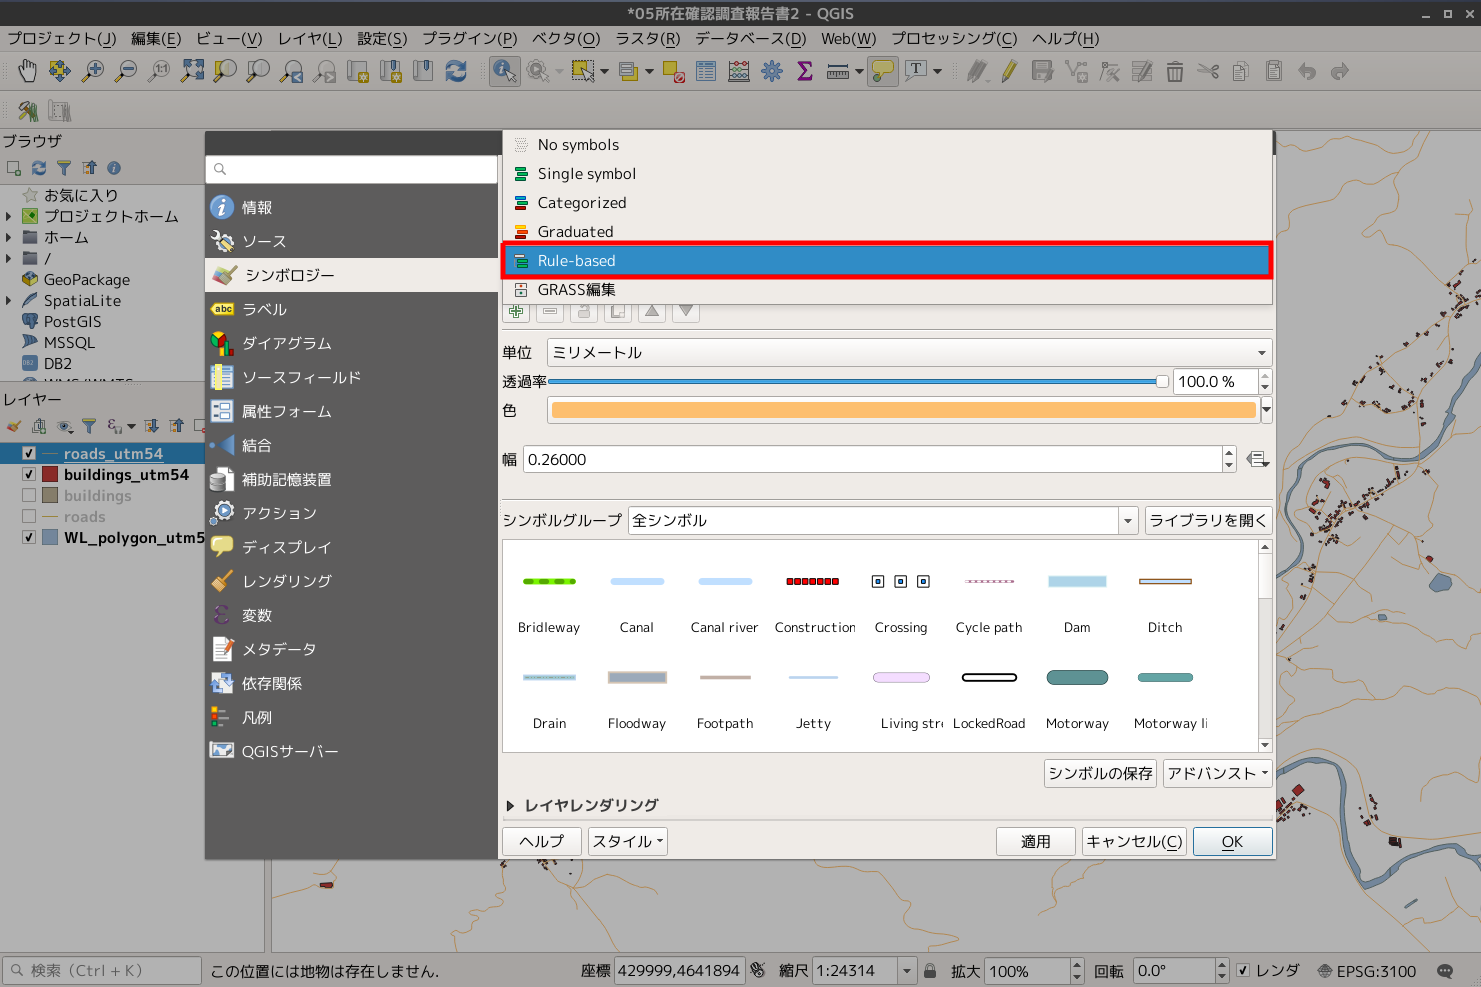
\includegraphics[width=1\linewidth]{09.png}
\caption{「Ruleーbased」に切り替える}
\end{figurehere}

\begin{figurehere}
\centering
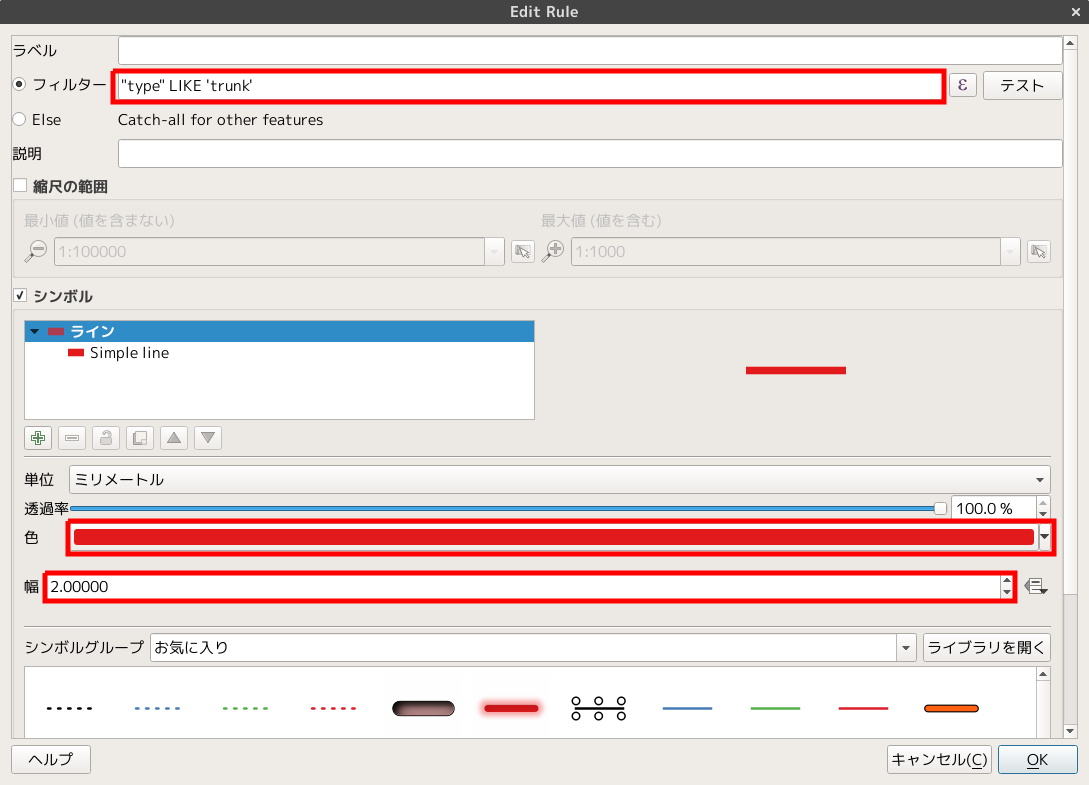
\includegraphics[width=1\linewidth]{11.png}
\caption{論理式で地物を選択して線種と色を指定する}
\end{figurehere}

\begin{figurehere}
\centering
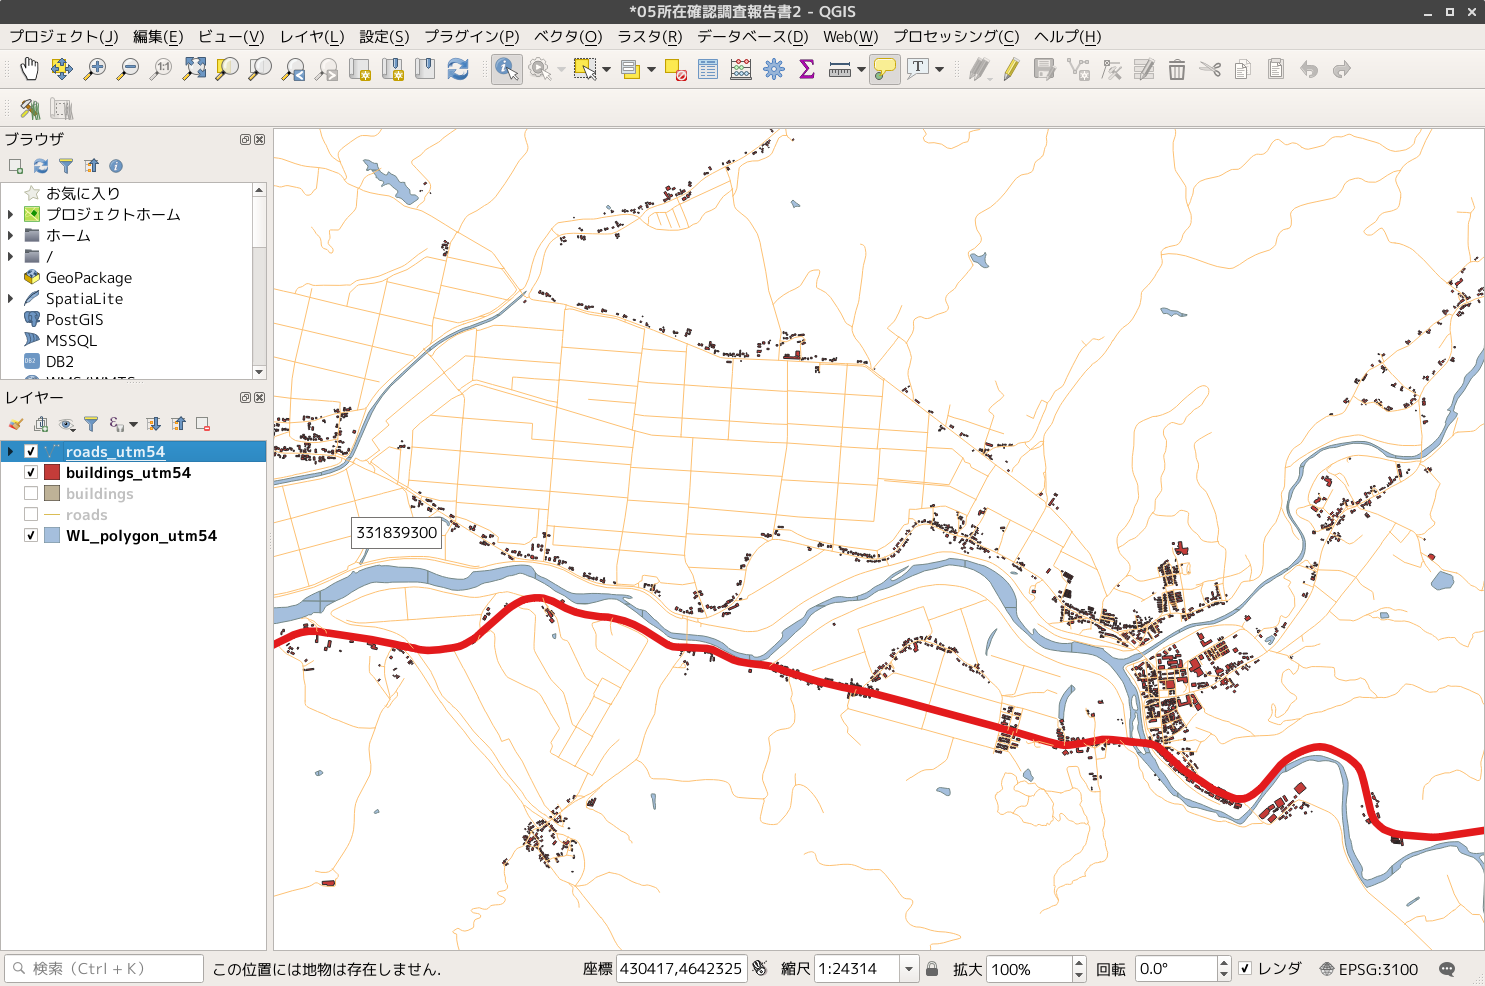
\includegraphics[width=1\linewidth]{12.png}
\caption{国道だけを赤く塗る}
\end{figurehere}

%%%%
\section{論理式のルール}
論理式のルールとして以下は必須です。覚えてください。

\begin{itemize}
\item 演算子「LIKE」は「=」とほぼ同じ働きをするマッチング演算子
\item フィールド名は「""」で囲む
\item フィールド値(文字列)は「''」で囲む
\item ワイルドカードは「\%」
\end{itemize}

\begin{itembox}[l]{論理式の例}
「type」フィールドの「trunk」を検索

\begin{center} "type"  LIKE 'trunk' 
\end{center}  

「type」フィールドの「tru〜」を検索

\begin{center}  "type"  LIKE 'tru\%'
\end{center}

「type」フィールドの「trunk」と「primary」を検索

\begin{center}  "type"  LIKE 'trunk' OR "type"  LIKE 'primary'
\end{center}

「type」フィールドが「trunk」で「name」フィールドに「函館」を含むものを検索

\begin{center}   "type"  LIKE 'trunk' AND "name"  LIKE '\%函館\%'
\end{center}
\end{itembox}

%%%%
\section{スタイルのロード}
あらかじめ作成した論理式や描画条件を保存して読み込むことができます\footnote{今回使用するスタイルファイルは北海道庁喜多耕一さん作成のスタイルファイルです}。

\begin{figurehere}
\centering
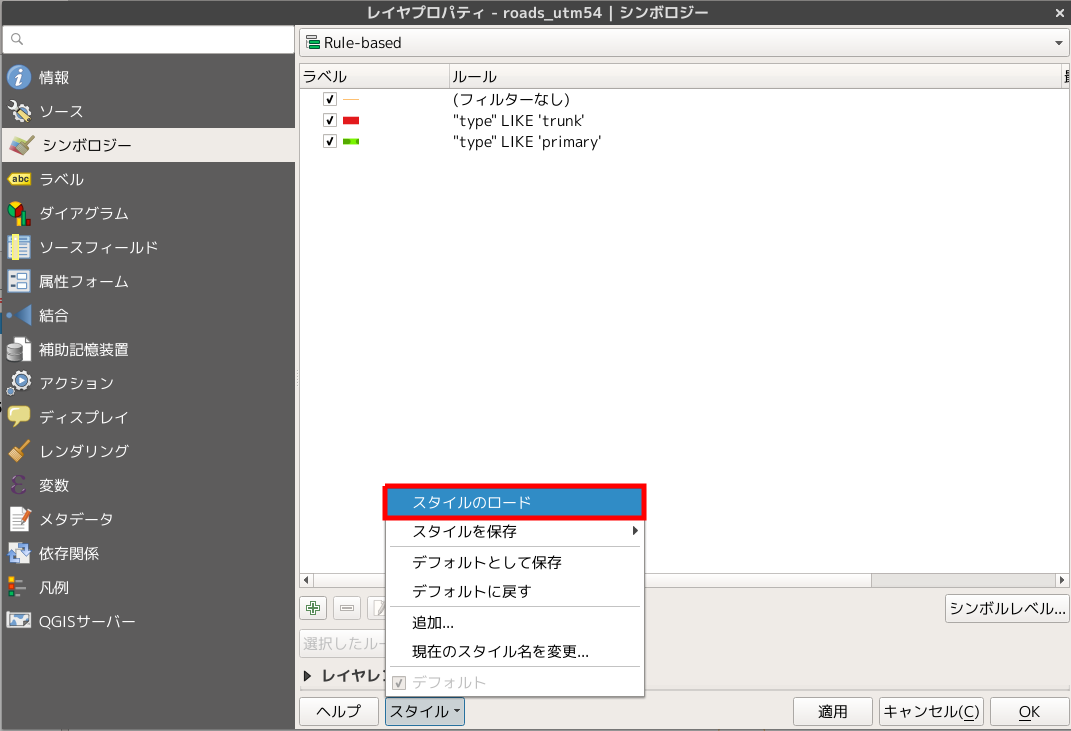
\includegraphics[width=1\linewidth]{16.png}
\caption{あらかじめ準備していたスタイルファイルを読み込む}
\end{figurehere}

\begin{figurehere}
\centering
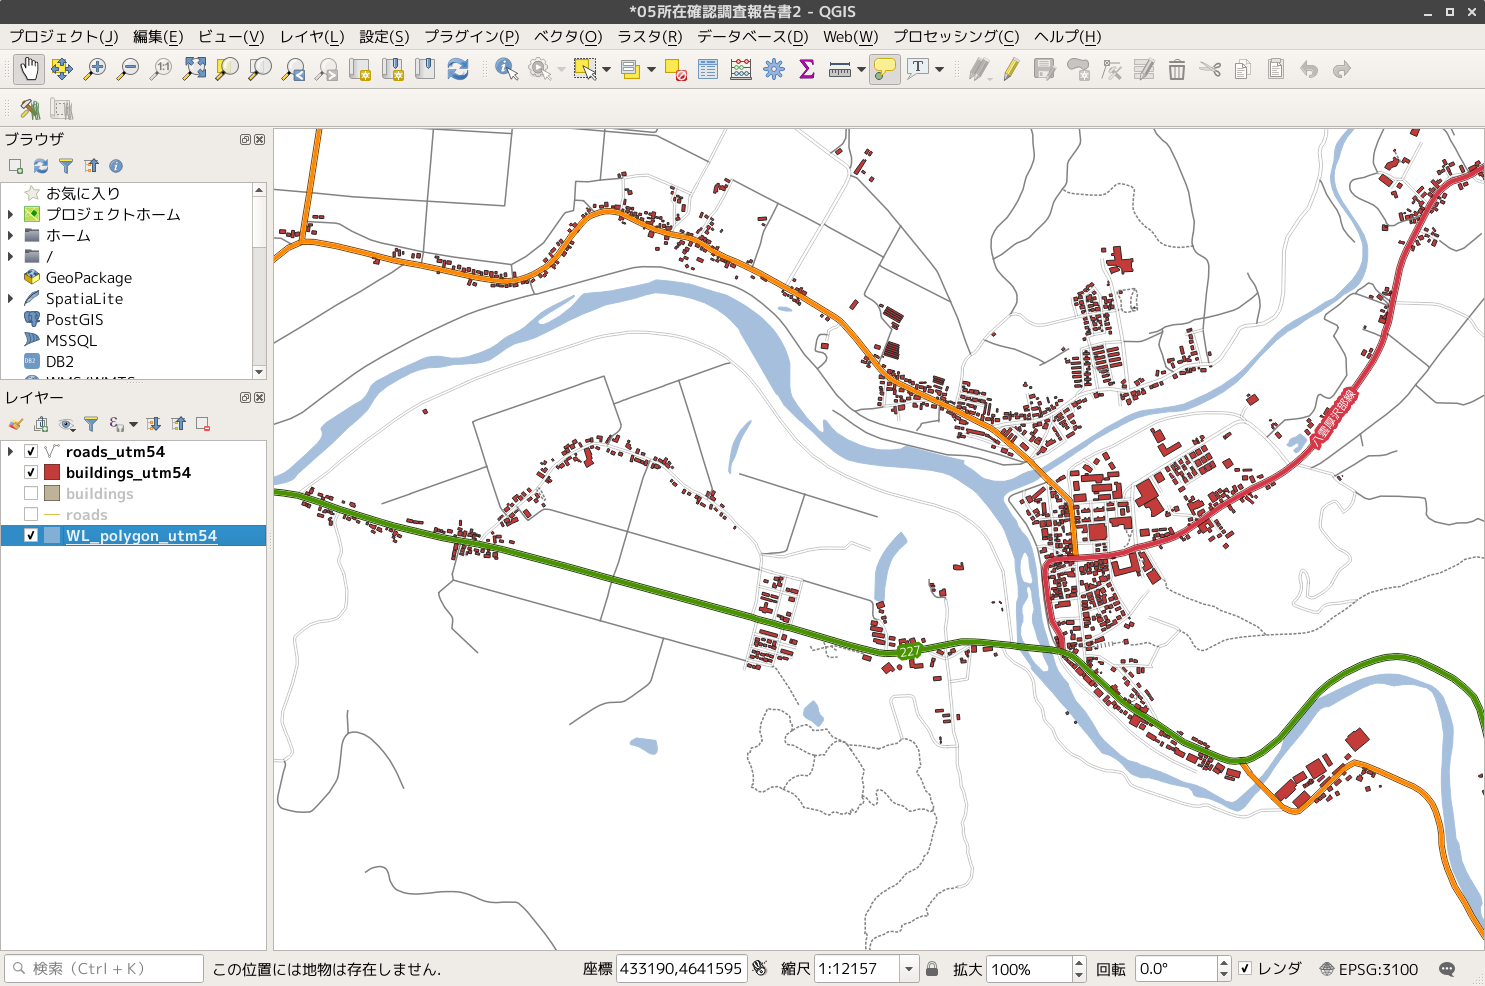
\includegraphics[width=1\linewidth]{18.png}
\caption{「マップリンク風」に描画された道路}
\end{figurehere}

%%%%
\section{自由自在に印刷する}
QGISでは印刷原稿作成に特化したブラウザ(「レイアウト」)が用意されています。「レイアウト」では複数の地図やスケール、方位記号、テキスト、凡例などを付け加えることができます。

\begin{figurehere}
\centering
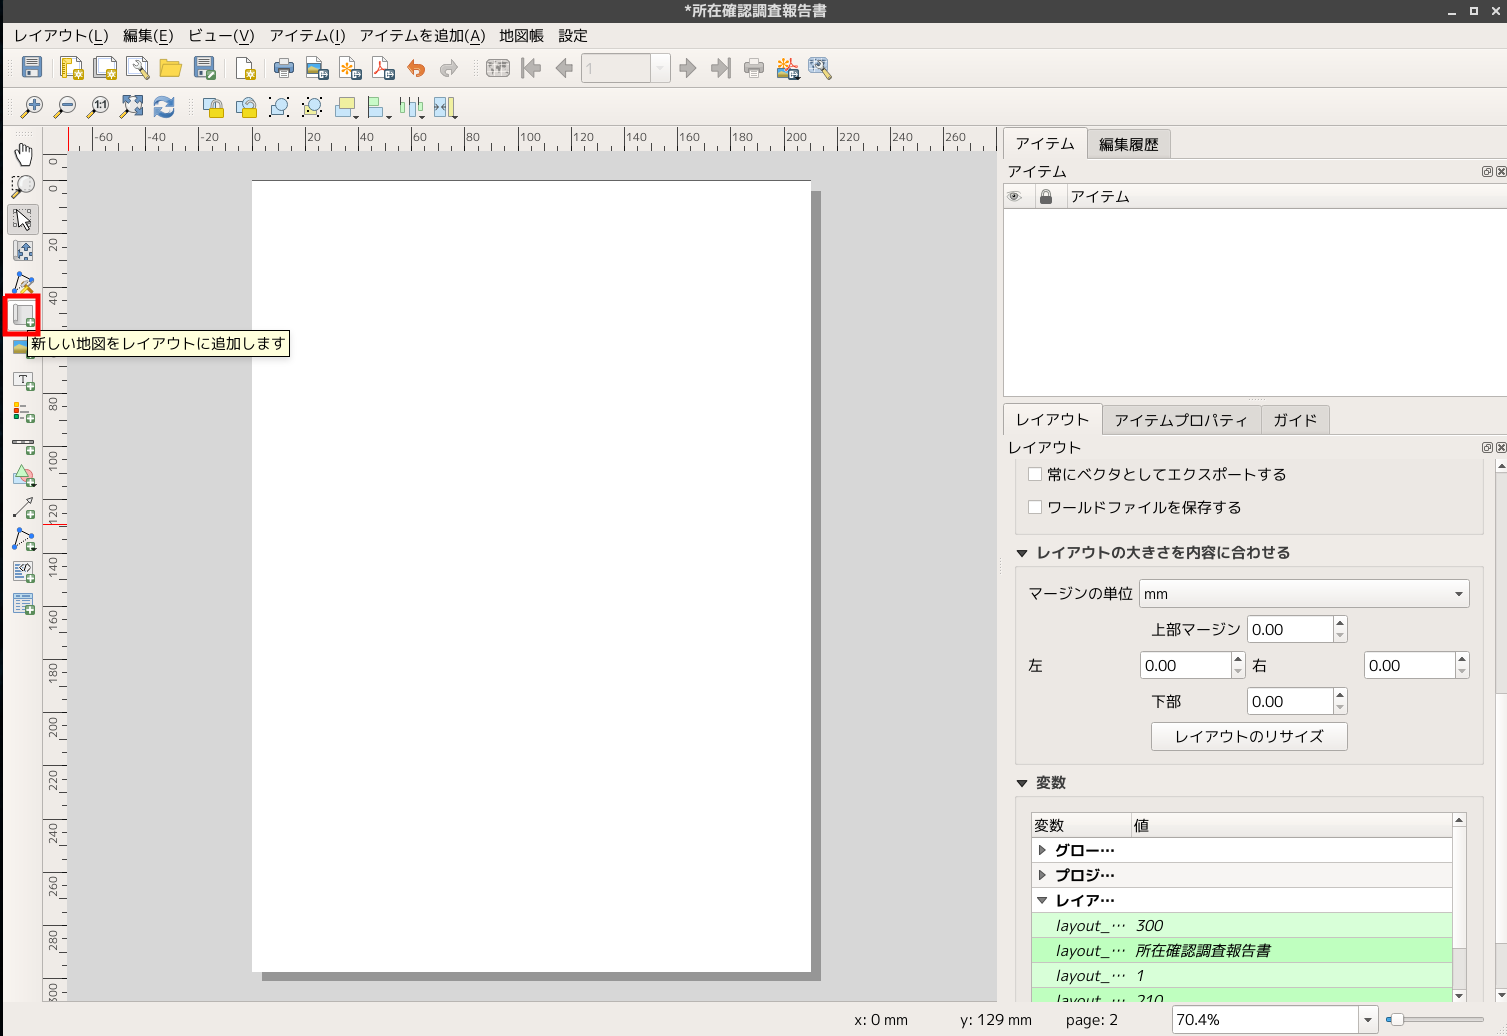
\includegraphics[width=1\linewidth]{31.png}
\caption{「レイアウト」を開く}
\end{figurehere}

%%%%
\section{地図を追加する}
地図をはじめとしたアイテムはドラッグで追加します。サイズは後からいくらでも調整できます。イラストレーターのような自由度はありませんが、ワードやエクセルの作図よりははるかに融通がききます。

\begin{figurehere}
\centering
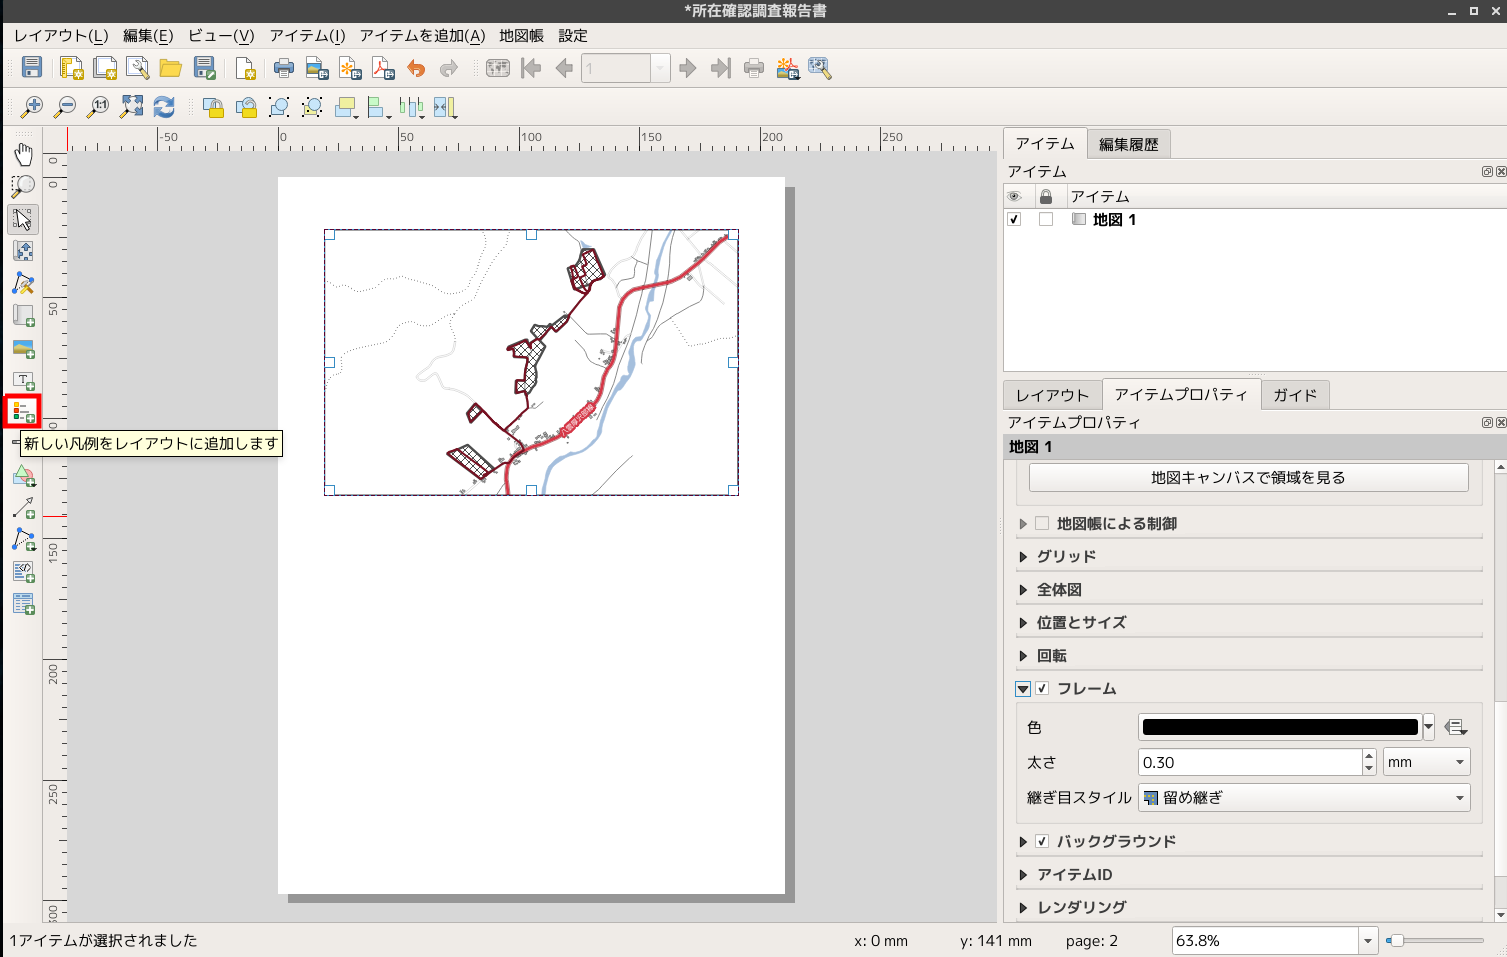
\includegraphics[width=1\linewidth]{36.png}
\caption{地図を追加する}
\end{figurehere}

%%%%
\section{凡例とスケールを追加する}
\begin{figurehere}
\centering
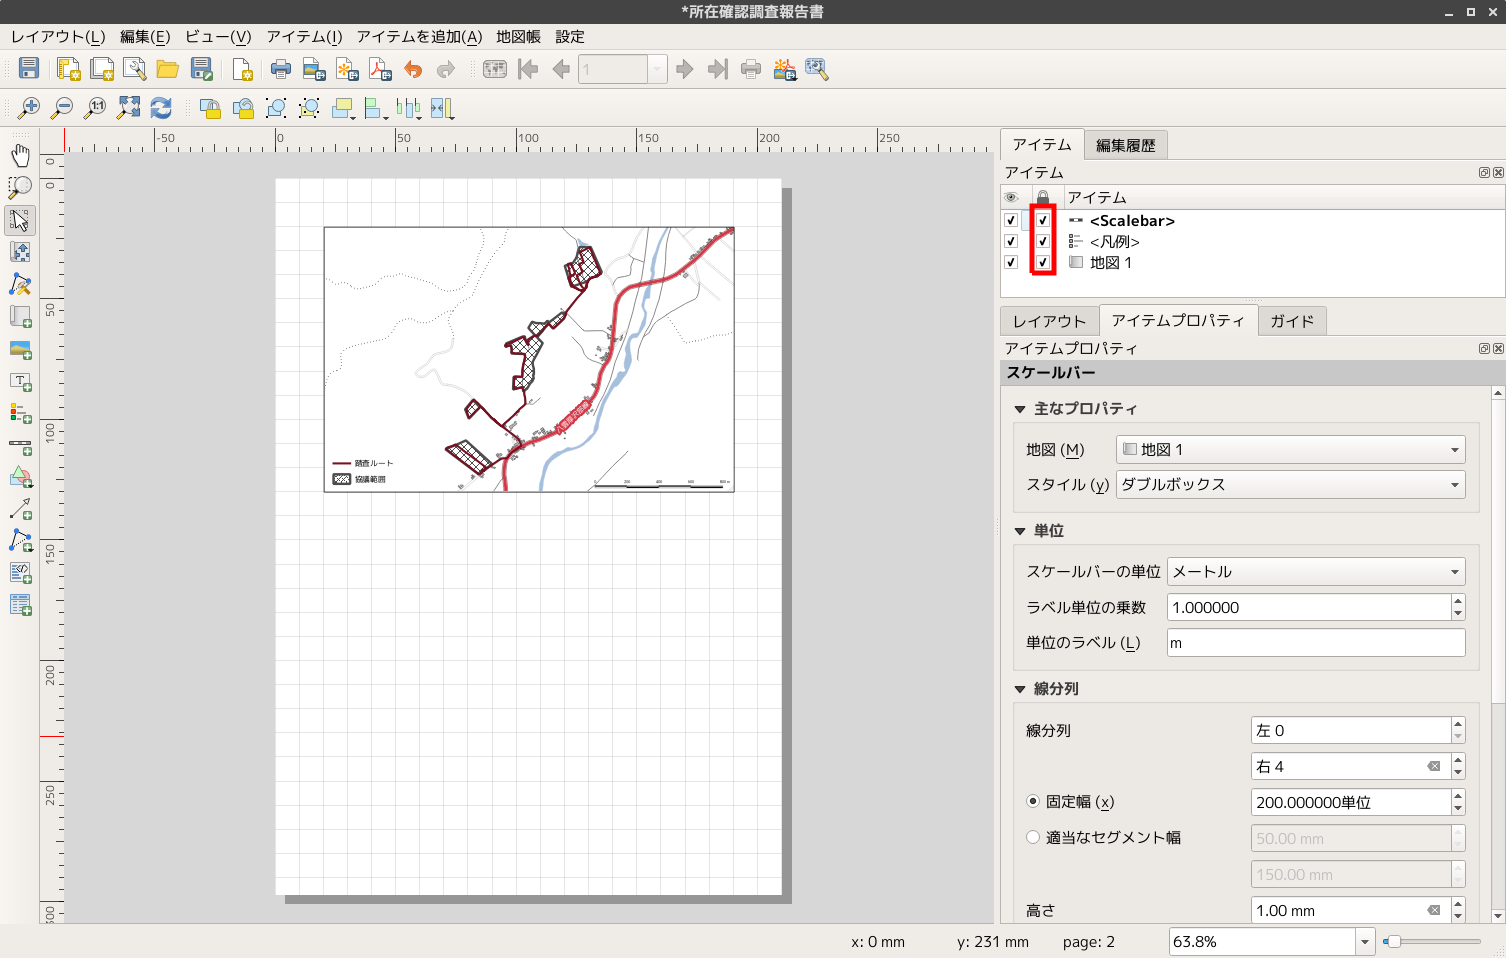
\includegraphics[width=1\linewidth]{46.png}
\caption{凡例とスケールを追加する}
\end{figurehere}

%%%%
\section{全体図を追加する}
\begin{figurehere}
\centering
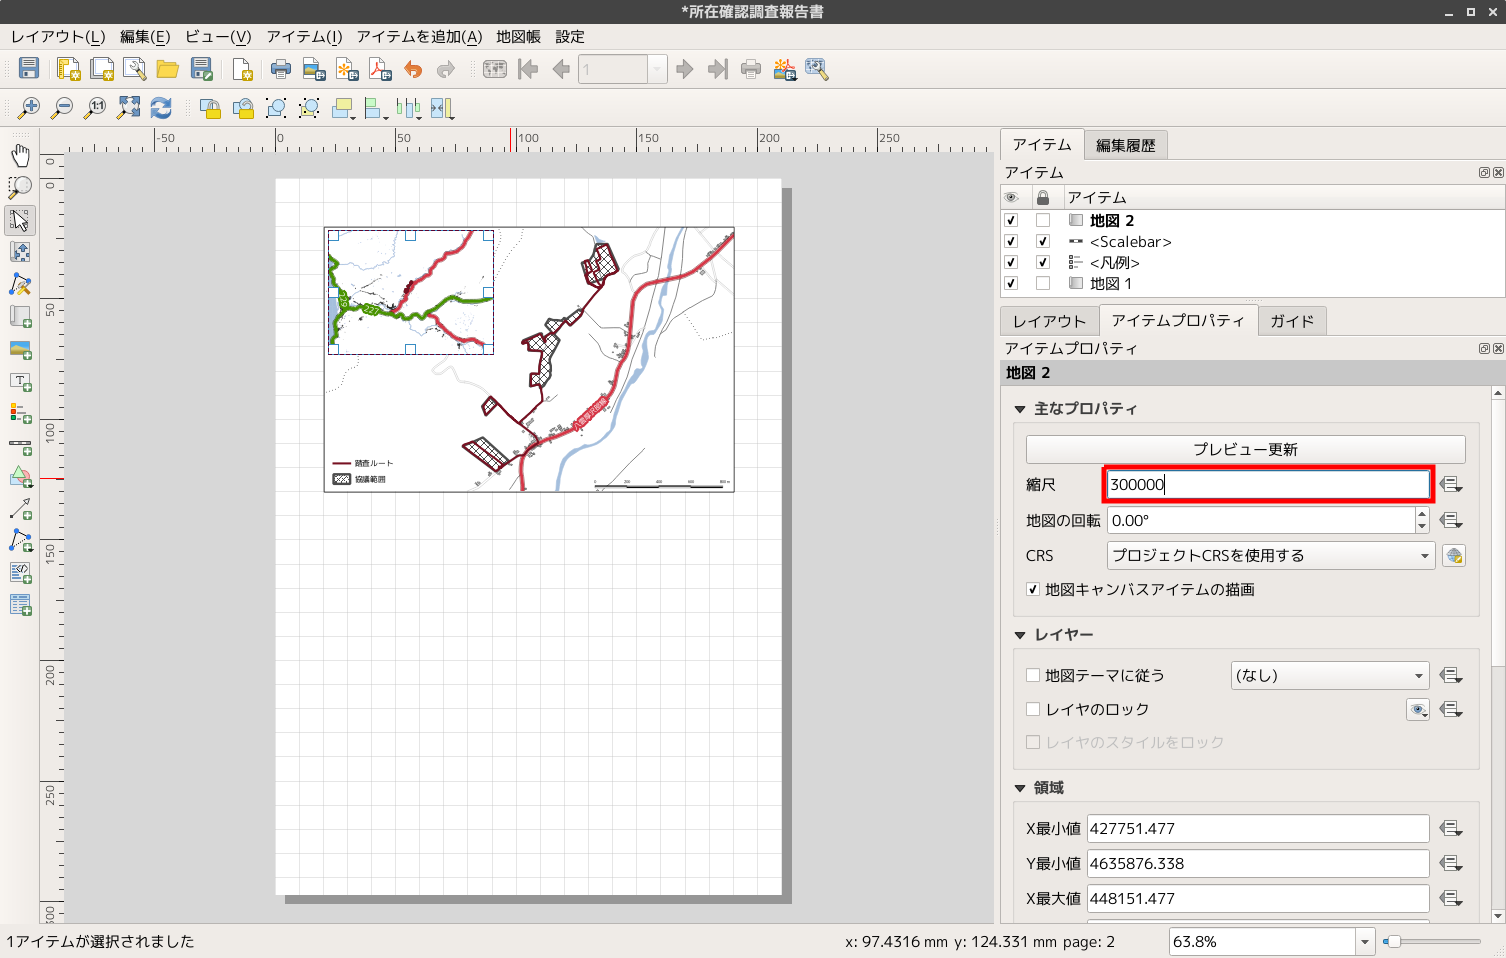
\includegraphics[width=1\linewidth]{48.png}
\caption{縮尺の違う別の地図を追加する}
\end{figurehere}

%%%%
\section{図形やテキスト、写真を追加する}
\begin{figurehere}
\centering
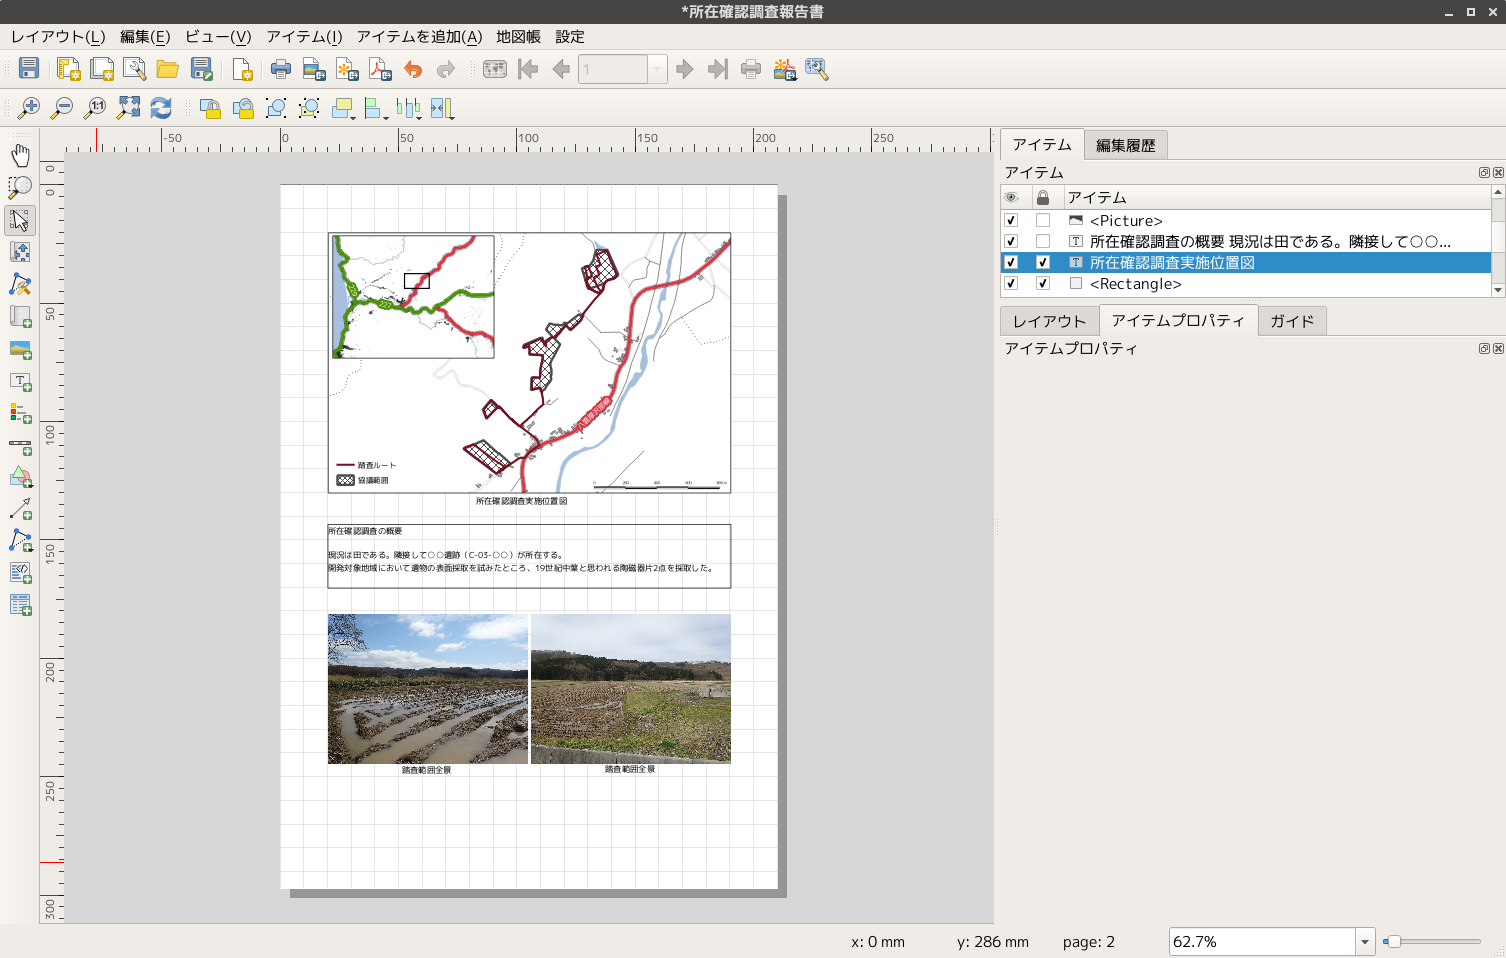
\includegraphics[width=1\linewidth]{57.png}
\caption{図形、テキスト、写真の追加}
\end{figurehere}

%%%%
\section{ラベルの自動表示}
\begin{figurehere}
\centering
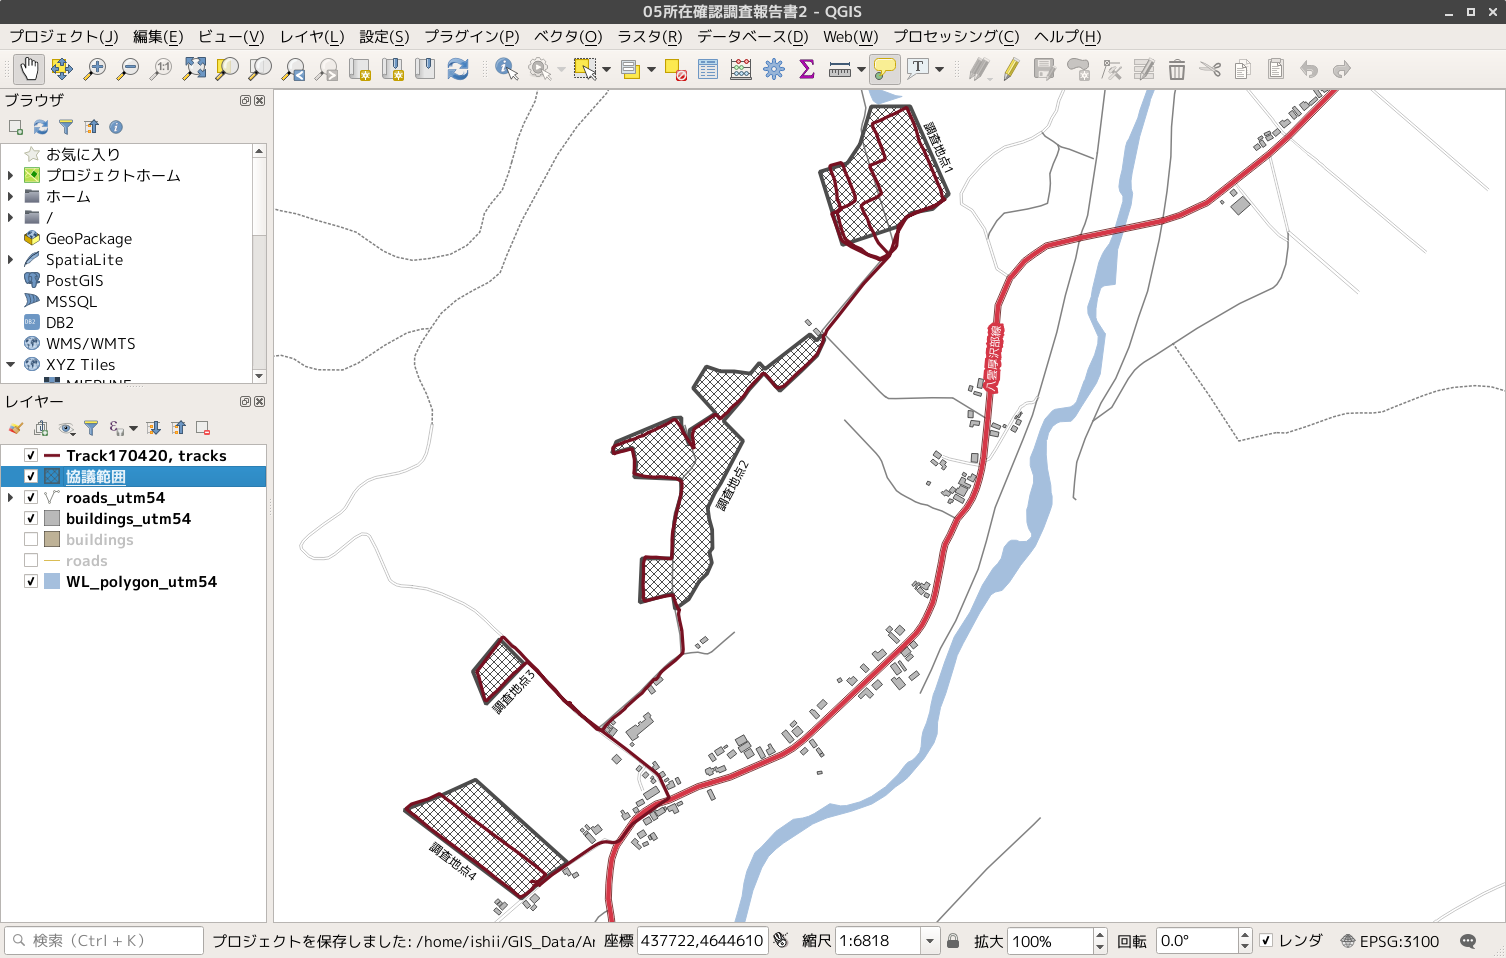
\includegraphics[width=1\linewidth]{62.png}
\caption{データベースから引用したラベルの表示}
\end{figurehere}

%%%%
\section{複数の地図を自動的に生成する}
調査地点が複数ある場合では同じ体裁の地図を地点を変えて何枚も出図することがあります。地図帳機能を使うと複数の地点の地図を一括で作成することができます。また、図表名称などをデータベースの値から引用することができるので、GISのデータベース機能を有効に利用することができます。

\begin{enumerate}
\item 地図帳」→「地図帳の設定」
\item 「地図帳」タブ
\item 「地図帳を作成する」をクリック
\item 「被覆レイヤ」→「協議範囲」
\item  地図を選択
\item  「アイテムプロパティ」タブ→「地図帳による制御」
\item  「地物周りの余白」→「100\%」
\end{enumerate}

\begin{figurehere}
\centering
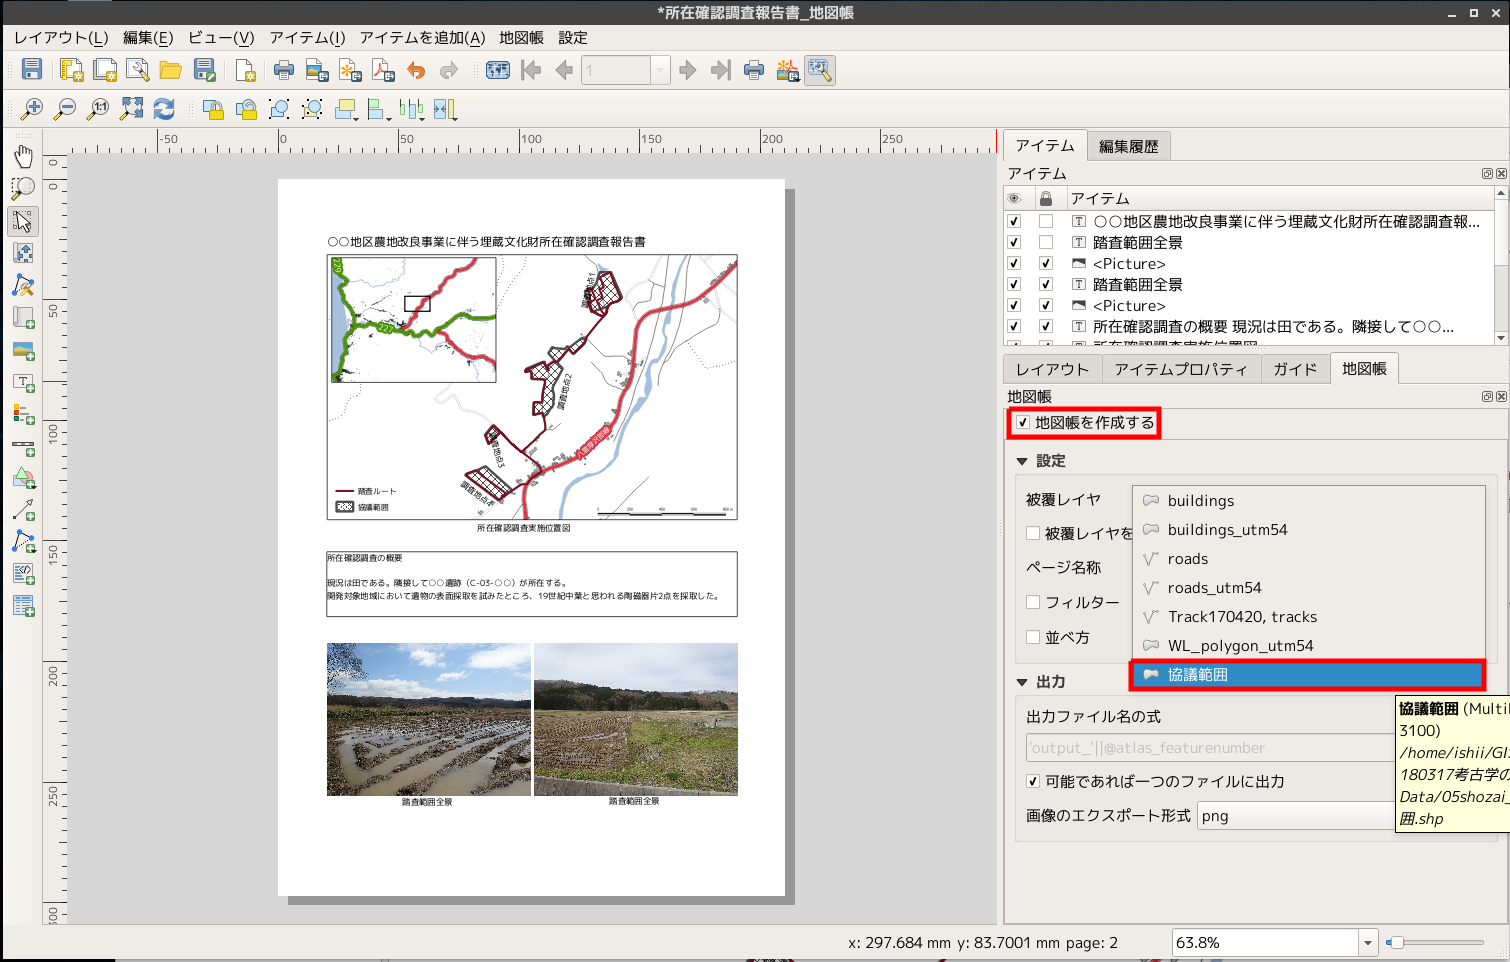
\includegraphics[width=1\linewidth]{66.png}
\caption{「被覆レイヤ」で自動生成する地図を決める}
\end{figurehere}

\begin{figurehere}
\centering
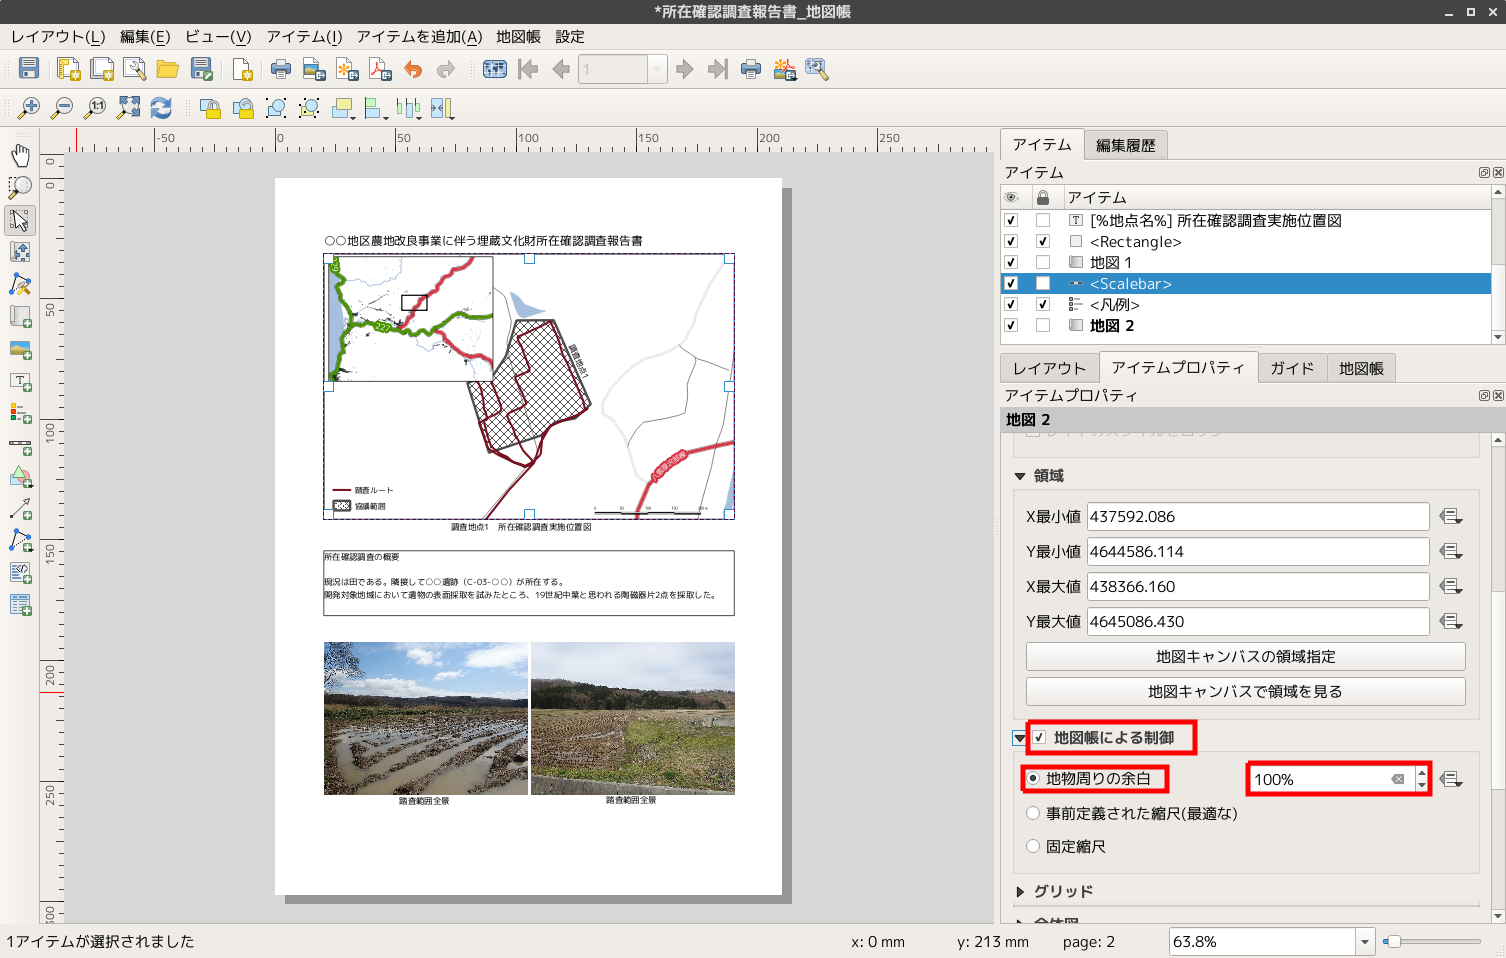
\includegraphics[width=1\linewidth]{68.png}
\caption{印刷する領域を自動的に決める}
\end{figurehere}

%%%%
\section{テキストをデータベースから自動的に引用する}

テキストボックスの中に以下のように入力すると「被覆レイヤ」で選択したレイヤの「地点名」フィールドの値が自動的に表示される。

[\%地点名\%] 所在確認調査実施位置図

\begin{figurehere}
\centering
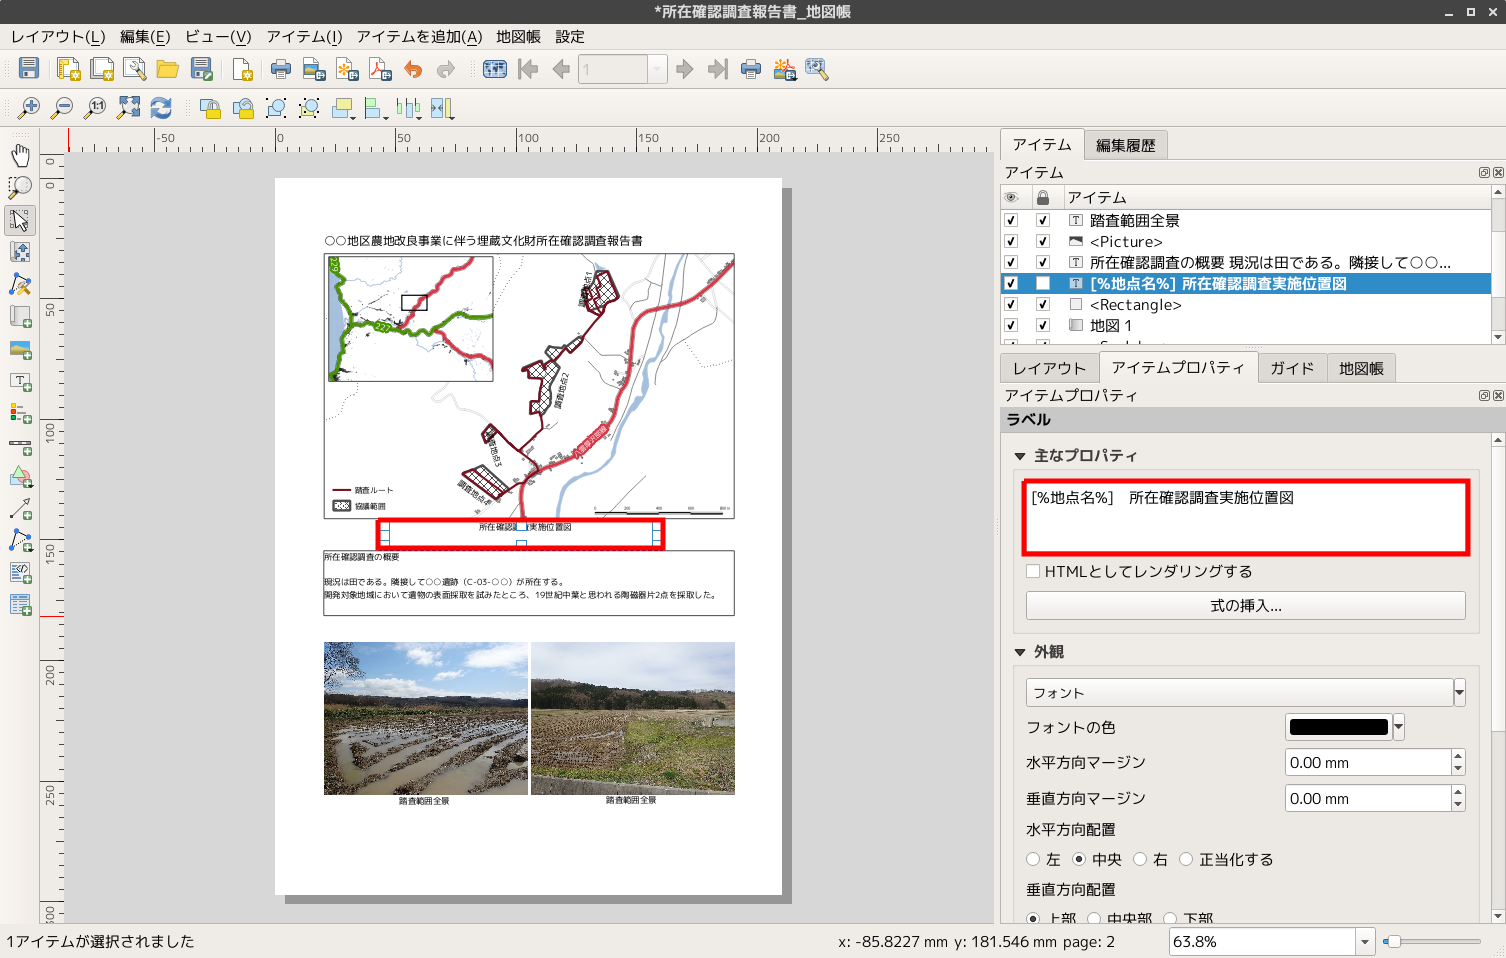
\includegraphics[width=1\linewidth]{67.png}
\caption{テキストの自動表示を設定する}
\end{figurehere}

%%%%
\section{複数の地図をまとめてPDF出力}

\begin{enumerate}
\item 「地図帳」→「地図帳のプレビュー」
\item 「地図帳のエクスポート」→「PDFとしてエクスポート」
\end{enumerate}

\begin{figurehere}
\centering
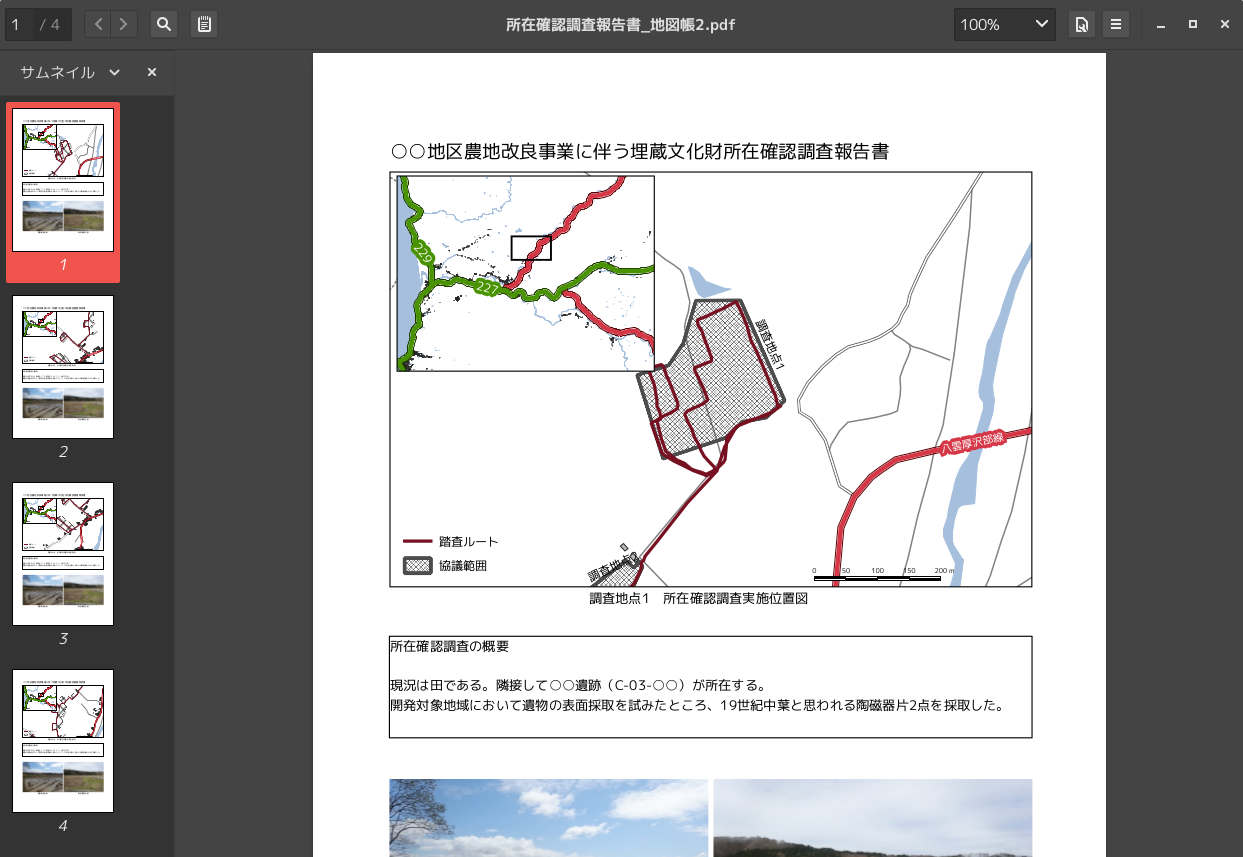
\includegraphics[width=1\linewidth]{71.png}
\caption{複数地点の所在報告書を一括してPDF出力}
\end{figurehere}

\section{データと著作権と測量法}
本研修で使用した道路データ(OpenStreetMap)は通常著作物とはみなされません。一方、作成した地図画像(スタイルファイル含む)は著作物となりえます。一般的なウェブ地図(GoogleMapなど)は地図画像ですから、著作権法の適用を受けるのでスクリーンショットなどによる利用(複製や公衆送信)については著作者が定めたルールにしたがって許諾等を受けることとなります。

国土地理院発行の地図を報告書に掲載する場合に承認が必要な場合があります。こうした制限は測量法によるものです。測量法は測量の重複を防ぎ正確性を確保することを目的とした法令です。注意が必要なのは「地図の調整」も「測量」に含まれることです。

本研修では地理院のデータを使用して地図画像を作成しましたが、こうした地図画像の調整は測量法上の「測量」にあたる行為\footnote{
地理院のデータを使用して新たに地図を作成する行為は法第30条の「測量成果の使用」に該当します。
}
です。

また、今回の研修では地理院データを受講者の方々に配布しましたが、この行為は「測量」にあたりませんので測量法の適用を受けません。

以上のように、地図データを扱うためには著作権法上の取り扱いと測量法上の取り扱いを理解する必要があります。ルールにしたがって必要な手続きを行ってください。



%\end{multicols}
\end{document}
